\documentclass[10pt,twocolumn]{article}
\usepackage{mathptmx} 
\usepackage{amsmath}
\usepackage{amssymb}
\usepackage{graphicx}
\usepackage{xcolor}
\usepackage{hyperref}
\usepackage{lipsum} 
\usepackage{subcaption}
\usepackage{siunitx}
\usepackage{booktabs}
\usepackage{algorithm}
\usepackage{algpseudocode}
\usepackage{stfloats} 

% Set the paper margins
\usepackage[margin=1in]{geometry}
\usepackage{adjustbox}
% Set the line spacing
\renewcommand{\baselinestretch}{1}
% Set the title and authors
\title{\textbf{\textsc{Drought Analysis Using Sentinel-2 Satellite Data}}}
\author{
  \textbf{Andrea Borghesi} \\
    $916202$ \\
  a.borghesi1@campus.unimib.it
}
\date{}

% Customize section headings
\usepackage{titlesec}
\titleformat{\section}{\large\bfseries\scshape\color{black}}{\thesection}{1em}{}
\titleformat{\subsection}{\bfseries}{\thesubsection}{1em}{}
\begin{document}

\twocolumn[
  \begin{@twocolumnfalse}
    \maketitle
  \end{@twocolumnfalse}
]

\section{Introduction}
This project evaluates the drought conditions based on Sentinel-2 satellite data. Drought is a natural hazard that affects ecosystems and agricultural and water resources. Through remote sensing technology, as satellite imagery, we can provide necessary information to monitor environmental changes over large areas.

For this research, two areas were selected: the "Riserva Naturale Pizzo Cane, Pizzo Trigna, Grotta Mazzamuto" around Palermo in Sicily, which serves as the case study area, and the "Parco Fluviale del Tevere" in Latium, as the control area. The case study area has been chosen due the alarming drought conditions in Sicily, while the control area has been chosen as been notably less affected by drought during the study period.

This research study will focus on analyzing various types of spectral indices derived from Sentinel-2 imagery, such as the Normalized Difference Water (NDWI) Indexes by Gao and McFeeters, the Moisture Stress Index (MSI), Normalized Difference Moisture Index (NDMI), and Modified Soil Adjusted Vegetation Index 2 (MSAVI2). 
These indices provide information about vegetation health, water availability, and moisture stress; all important parameters for drought condition assessment.

The K-Means++ algorithm groups pixels with similar spectral characteristics into clusters. 

The distribution of these clusters over several years is analyzed to identify spatial and temporal patterns indicative of drought.

The project is organized into three main stages: data collection, data processing, and data analysis. The data collection phase consists in collecting Sentinel-2 satellite imagery. During the data processing phase, we compute spectral indices, applying water and urban masks, and conduct K-Means clustering to our data structure. Lastly, data analysis will look into cluster distribution correlating them with drought conditions.
\section{Materials and Methods}
\subsection{Study Areas}

\textbf{Case Study Area:} The case study area is the "Riserva Naturale Pizzo Cane, Pizzo Trigna, Grotta Mazzamuto" near Palermo, Sicily, Italy. This area, covering approximately \SI{90}{\kilo\meter\squared}, includes a natural lake, providing an opportunity to observe water body dynamics in response to drought.

\begin{figure}
  \centering
  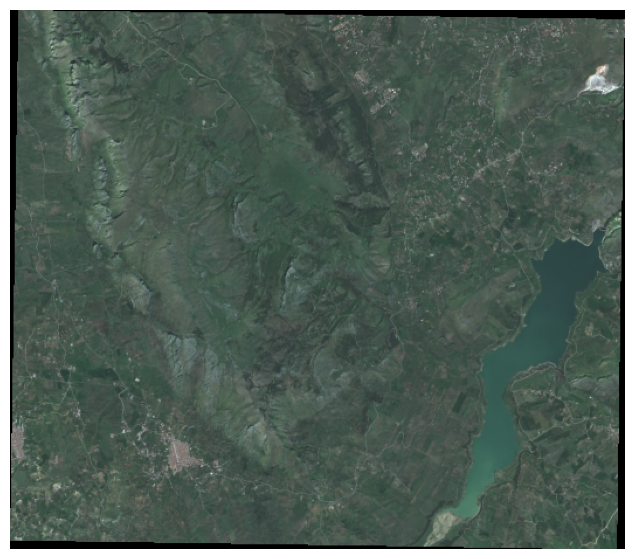
\includegraphics[width=0.5\textwidth]{images/case_palermo_april_2020_rgb.png}
  \caption{Case study Area of Interest: Riserva Naturale Pizzo Cane, Pizzo Trigna, Grotta Mazzamuto, Sicily - April 2020}
  \label{fig:case_rgb}
\end{figure}

\textbf{Control Area:} The control area is the "Parco Fluviale del Tevere" in Latium, Italy. This area, also covering about \SI{90}{\kilo\meter\squared}, includes a lake and is chosen for its potential to exhibit different responses to drought compared to the case study area.

\begin{figure}
  \centering
  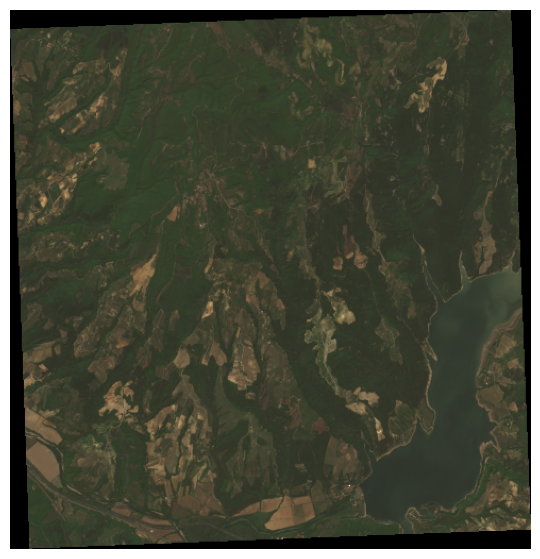
\includegraphics[width=0.5\textwidth]{images/control_tevere_april_2017_rgb.png}
  \caption{Control study Area of Interest: Parco Fluviale del Tevere, Latium - April 2017}
  \label{fig:control_rgb}
\end{figure}

\subsection{Data Collection}
Satellite data is collected from the Copernicus Open Access Hub, utilizing the Sentinel-2 satellite constellation \cite{wang2016fusion}. The dataset spans from 2017 to 2024, covering two distinct periods each year: April, representing a typically wetter period post-winter, and July, representing the peak of the dry season. The data used is preprocessed to Level-2A, indicating that atmospheric corrections have already been applied.

The collected data is in the form of raster images with a spatial resolution of 20 meters per pixel. Each pixel contains values for 13 spectral bands. For this study, bands 4 (Red), 8A (Near Infrared), 11 (Shortwave Infrared), and 12 (Shortwave Infrared) are primarily used. Cloud coverage is a crucial consideration, and only images with at most 5\% cloud coverage are selected to minimize data quality issues.

\subsection{Spectral Indices Calculation}
The following spectral indices are calculated from the Sentinel-2 data:

\begin{itemize}
    \item \textbf{Normalized Difference Water Index (NDWI - Gao) \cite{gao1996ndwi}:}
    \begin{equation*}
    \text{NDWI} = \frac{B8A - B11}{B8A + B11}
    \end{equation*}
    Used to monitor changes in water content of vegetation.
    \item \textbf{Normalized Difference Water Index (NDWI - McFeeters) \cite{mcfeeters1996use}:}
    \begin{equation*}
    \text{NDWI}_{\text{McFeeters}} = \frac{B03 - B8A}{B03 + B8A}
    \end{equation*}
    Specifically used for water body detection and creating the water mask.
    \item \textbf{Moisture Stress Index (MSI):}
    \begin{equation*}
    \text{MSI} = \frac{B11}{B8A}
    \end{equation*}
    Indicates vegetation water stress.
    \item \textbf{Normalized Difference Moisture Index (NDMI):}
    \begin{equation*}
    \text{NDMI} = \frac{B8A - B12}{B8A + B12}
    \end{equation*}
    Sensitive to the moisture levels in vegetation.
    \item \textbf{Modified Soil Adjusted Vegetation Index 2 (MSAVI2):}
    \begin{align*}
      \text{MSAVI2} &= \frac{1}{2} \Big( 2(B8A + 1) \\
      &\quad - \sqrt{(2 \times B8A + 1)^2 - 8 \times (B8A - B04)} \Big)
    \end{align*}
      
    Used to assess vegetation health while minimizing soil background effects, used also for masking urban areas.
\end{itemize}

\subsection{Data Processing}
The data processing phase involves several key steps to transform raw satellite imagery into meaningful representations of drought conditions. These steps are detailed in Algorithm \ref{alg:data_prep} and Algorithm \ref{alg:clustering} and are described below.

We first fix the study area location and month, and then extract the relevant Sentinel-2 bands for the spectral indeces computation, for each year within the study period. The spectral indices are calculated for each image, and a multi-channel raster is created with the spectral indices as channels. This process is repeated and concatenated for all years along a new dimension, namely the years dimension. This results in a tensor of shape (years, height, width, channels) that contains the spectral index data for the study area over the study period.

Before proceeding to cluster analysis, a water mask is created using the McFeeters version of the NDWI, specifically designed for water body delineation. A threshold of 0 is applied to the NDWI values, effectively identifying pixels representing water within the study areas. In a similar way we also apply an urban mask by applying a threshold to MSAVI2 of 0.25. The water mask is then used to exclude water pixels from the subsequent analysis, ensuring that the clustering process focuses on land features and their drought-related characteristics.

The core of the data processing involves the application of the K-Means++ \cite{huang2014extensions} clustering algorithm to the first four spectral indices combined, namely: NDWI (Gao), MSI, NDMI, MSAVI2. This unsupervised learning technique groups pixels with similar spectral signatures into clusters, revealing spatial patterns (within the spectral indexes space) in the data that can be related to different levels of drought severity. To determine the optimal number of clusters, the Elbow method is employed. This method helps to identify the number of clusters that best balances the within-cluster variance and the complexity of the model.

Once the K-Means++ algorithm has identified the clusters, a crucial step is to sort the cluster labels to ensure consistency and interpretability across different years. The clusters are sorted based on their mean NDMI and NDWI values in ascending order. This means that lower cluster numbers (e.g., Cluster 1) will generally correspond to areas with lower moisture content and higher vegetation stress (drier conditions), while higher cluster numbers will represent areas with higher moisture content and healthier vegetation (wetter conditions). The sorting is performed globally across all years, fixing the study area and month, to maintain consistency in cluster labeling throughout the study period.

To further refine the analysis and account for the presence of water bodies, a special cluster label (k, since we start numbering from 0, where k is the number of clusters) is manually assigned to all pixels identified as water by the water mask. This allows for the explicit tracking of changes in water body extent over time, which can be an important indicator of drought in itself. The cluster distributions, representing the proportion of pixels assigned to each cluster, are then calculated for each year. 
% Finally, to understand the relationships between the clusters, an inter-cluster distance matrix is computed. This matrix quantifies the dissimilarity between cluster centers in the multi-dimensional spectral index space using the Euclidean distance, providing insights into the distinctness of the different land cover or moisture conditions represented by each cluster, and therefore the quality of the clustering itself.


\section{Results}
A first general note is that each image by nature is slightly tilted, and for technical reasons the extra space has not been removed and kept during clustering. This extra border values are always kept in the same cluster, namely cluster 0, and are not considered in the analysis.
A second note regards the water cluster, which is always the last cluster, and is considered only in some of the analysis, as this cluster has been added manually after the clustering process. This is due the fact that the pixel representing bodies of water would have had a very different spectral signature and would have been assigned to a cluster not representative of its actual wetness, being trivially the highest.
The elbow method is used to determine the optimal number of clusters and, for simplicity's sake we chose an homogeneous number across all studied locations and months. By analyzing the Within-Cluster Sum of Squares (WCSS) for each of these locations and months, we determine that a number of 6 clusters, one of which is dedicated for the border, is optimal for our analysis.

We start by analyzing the results in the month of April. A quick comparison of the rasterized labels of 2017 (Figure \ref{fig:case_april_lr_2017}) and 2024 (Figure \ref{fig:case_april_lr_2024}), shows evident signs of drought in the latter year, where we can see a significant shrinkage of the water body (Lake Caccamo). The cluster distribution of this study, displayed in Figure \ref{fig:case_april_clust_dist}, shows the same, with an overall increase of the drier clusters, namely 1, 2, and 3, and a decrease of the wetter clusters, 4, 5 and 6 (water cluster). Comparatively, the control area cluster distribution in the same month, displayed in Figure \ref{fig:control_april_clust_dist}, shows a more stable distribution of clusters in the first 4-5 years, with the exeption of 2017-18, where a significant decrease of cluster 5 is measured. The water cluster is stable across all years, showing no significant changes in the water body. There are nonetheless some significant instabilities within 2021-2024, where fluctuations in the distribution of clusters 2,3,4, and 5 are observed with no clear trend. 


Moving towards the July month analysis, starting with the case study area, we can again observe a significant shrinkage of the water body in 2024 compared to 2017, as shown in Figure \ref{fig:case_july_lr_2017} and Figure \ref{fig:case_july_lr_2024}. The cluster distribution in Figure \ref{fig:case_july_clust_dist} shows a much different trend compared to April. First and foremost, cluster 1, the driest, occupies a much bigger portion of the area, peaking in 2020 and 2024. If we momentarily exclude 2024, we can see an unexpected positive trend in every cluster: the wetter clusters, 4 and 5, show an overall, although slight, increase, while the drier clusters, after the 2020 dry peak, tend to decrease. The 2024 data and the water body shrinkage with cluster 6, however, abruptly invert this trend, with cluster 1 passing from less than $5\%$ in 2023 to an astonishing $~25\%$ in 2024. 

The control area, on the other hand, although significantly drier than its April counterpart, shows a much more stable and promising cluster distribution. With the wetter clusters, 4 and 5 overall increasing, cumulatively occupying more than $50\%$ of the area, and the drier clusters, 1, 2, and 3 slightly decreasing. The water cluster (6), as expected, remains stable across all years.



\section{Discussion}
The results of the cluster analysis, both of the case and control study area, provide valuable information regarding the current drought conditions. The results clearly highlights the difference in soil moisture content and vegetation health between the seasons, as expected.
The stability of the moisture and vegetation health condition is also clearly different between the seasons, with the July month showing a more stable condition compared to the April month. This is likely due to the fact that the April month is post-winter, where the vegetation is still recovering from the winter season, while the July month is during the peak of the dry season, where the vegetation has already adapted to the dry conditions.
We can also observe the significant shrinkage of the water body in the case study area, which is indicative of the alarming drought conditions. This is also confirmed by the cluster distribution analysis which shows, in both seasons, an increase in the drier clusters and a decrease in the wetter clusters, although the trend is not consistent across all years.
The control area, on the other hand, although of comparable stability across cluster distribution, the distribution itself is significantly different across both seasons, displaying the majority of the occupancy in the wetter clusters, indicating a healthier vegatation and soil moisture content. The water cluster, as expected, remains stable across all years, showing no significant changes in the water body.

\section{Conclusions}
In this study we have analyzed the drought conditions in two distinct areas using Sentinel-2 satellite data. The clustering of this processed data provided valuable insights regarding the moisture content and vegetation health of the mentioned areas. The results shows a clear evidence between the seasons, and between the drought conditions of the case and control study areas. The case study area particularly shows evident signs of drought, while the control area shows a much healthier condition. The results of this study can be used to monitor and assess the drought conditions in these areas, and to provide valuable information for drought management and mitigation strategies.

% Bibliography
\bibliographystyle{plain}
\bibliography{bibliography/references}

%----------------------------------------------------------
\onecolumn
\newpage
\appendix
\section{Figures \& Algorithms}
\begin{algorithm*}[h]
  \caption{Data Structure Preparation}
  \label{alg:data_prep}
  \begin{algorithmic}[1]
      \Require Location, Month, Years
      \State Initialize an empty list $yearly\_data$
      \For{each $year$ in $Years$}
          \State Retrieve Sentinel-2 images for $Location$ and $Month$
          \For{each raster image}
              \State Extract band data: B04, B08A, B11, B12, B03
              \State Calculate spectral indices: NDWI, MSI, NDMI, MSAVI2, NDWI (McFeeters)
              \State Create water mask based on NDWI (McFeeters) $>$ 0
              \State Create urban mask based on MSAVI2 $<$ 0.25 
              \State Apply water mask and urban to spectral indices
              \State Create multi-channel raster $R$ with spectral indices as channels
          \EndFor 
          \State Append $R$ to $yearly\_data$
      \EndFor
      \State Concatenate rasters in $yearly\_data$ along a new dimension to create tensor $data\_tensor$ of shape (years, height, width, channels)
      \State \Return $data\_tensor$
  \end{algorithmic}
\end{algorithm*}

\begin{algorithm*}[h]
    \caption{Clustering Algorithm}
    \label{alg:clustering}
    \begin{algorithmic}[1]
        \Require $data\_tensor$
        \State Determine optimal number of clusters $k$ using the Elbow method on $data\_tensor$
        \State Reshape $data\_tensor$ to 2D array of shape (years $\times$ height $\times$ width, channels)
        \State Apply KMeans++ algorithm to the reshaped data with $k$ clusters
        \State Get cluster labels $L$ for each pixel
        \State Sort labels globally using all years based on NDMI and NDWI (ascending)
        \State Reshape sorted labels $L$ to (years, height, width)
        \For{each year}
            \State Apply water mask to assign a special label (k+1) to water pixels
        \EndFor
        \State \Return Sorted cluster labels for each year
    \end{algorithmic}
\end{algorithm*}
\twocolumn

%----------------------------------------------------------

\begin{figure*}[h]
  \centering

  \begin{minipage}{1\columnwidth}
      \centering
      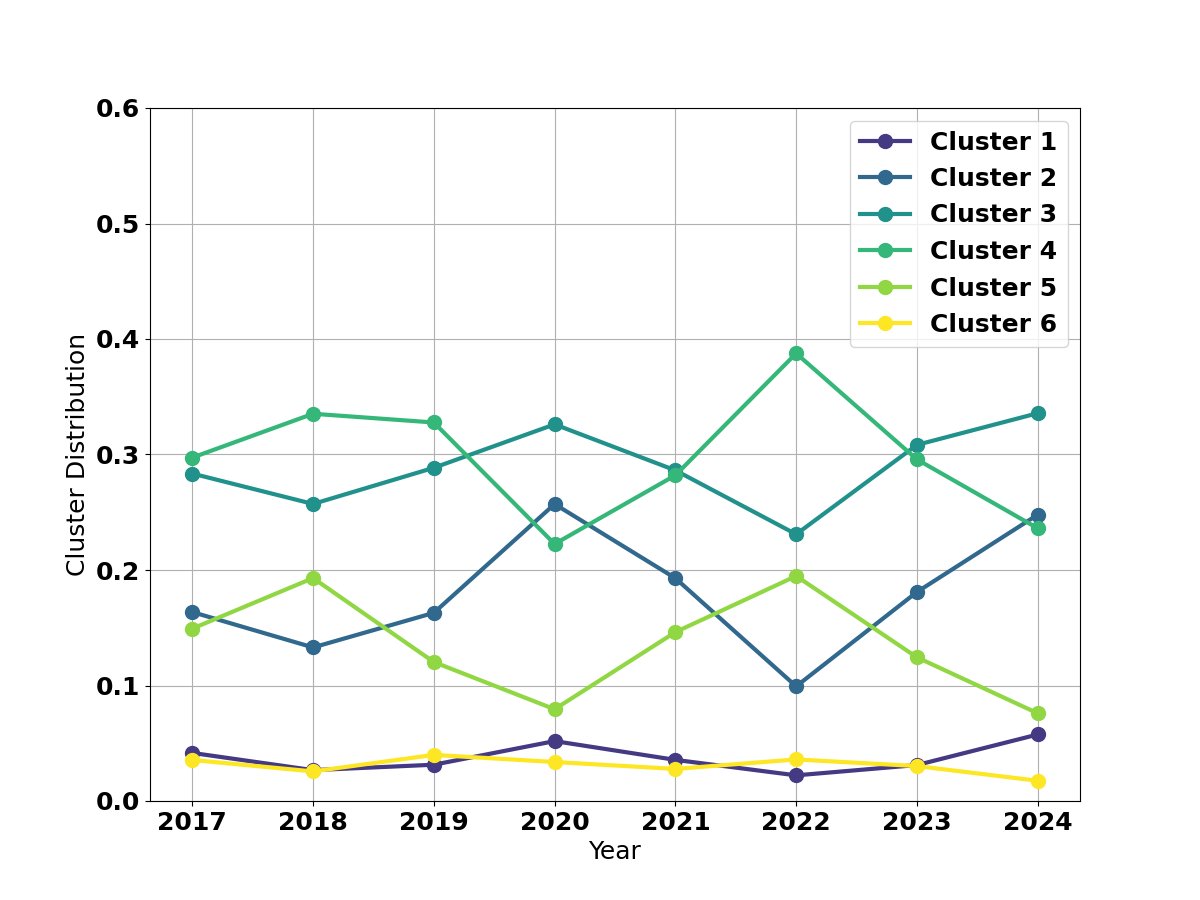
\includegraphics[width=\textwidth]{images/results/april/case/cluster_distribution_6_april.png}
      \caption{Case study - Cluster distribution in April 2017-2024} 
      \label{fig:case_april_clust_dist}
  \end{minipage}
  \hfill
  \begin{minipage}{1\columnwidth}
      \centering
      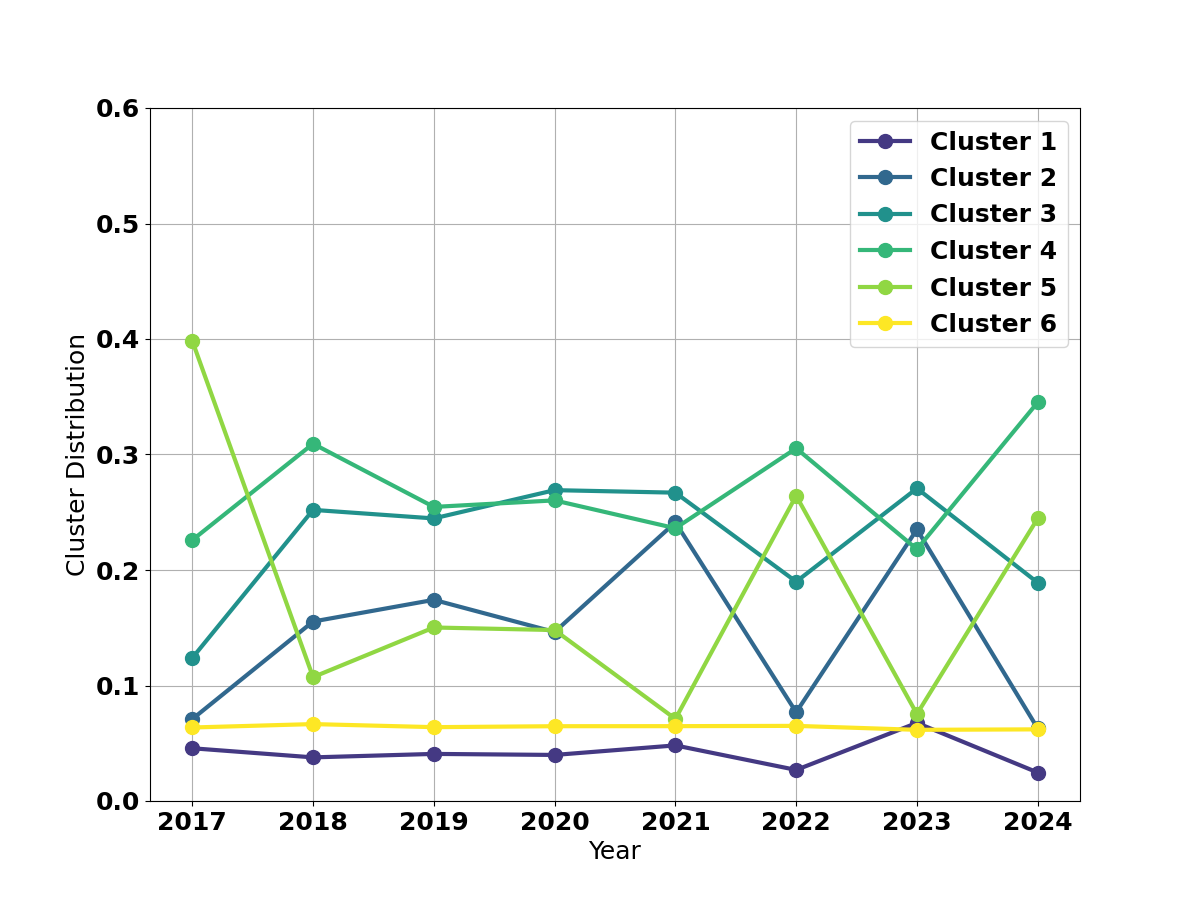
\includegraphics[width=\textwidth]{images/results/april/control/cluster_distribution_6_april.png}
      \caption{Control study - Cluster distribution in April 2017-2024}
      \label{fig:control_april_clust_dist}
  \end{minipage}

\end{figure*}


\begin{figure*}[h]
  \centering

  \begin{minipage}{1\columnwidth}
      \centering
      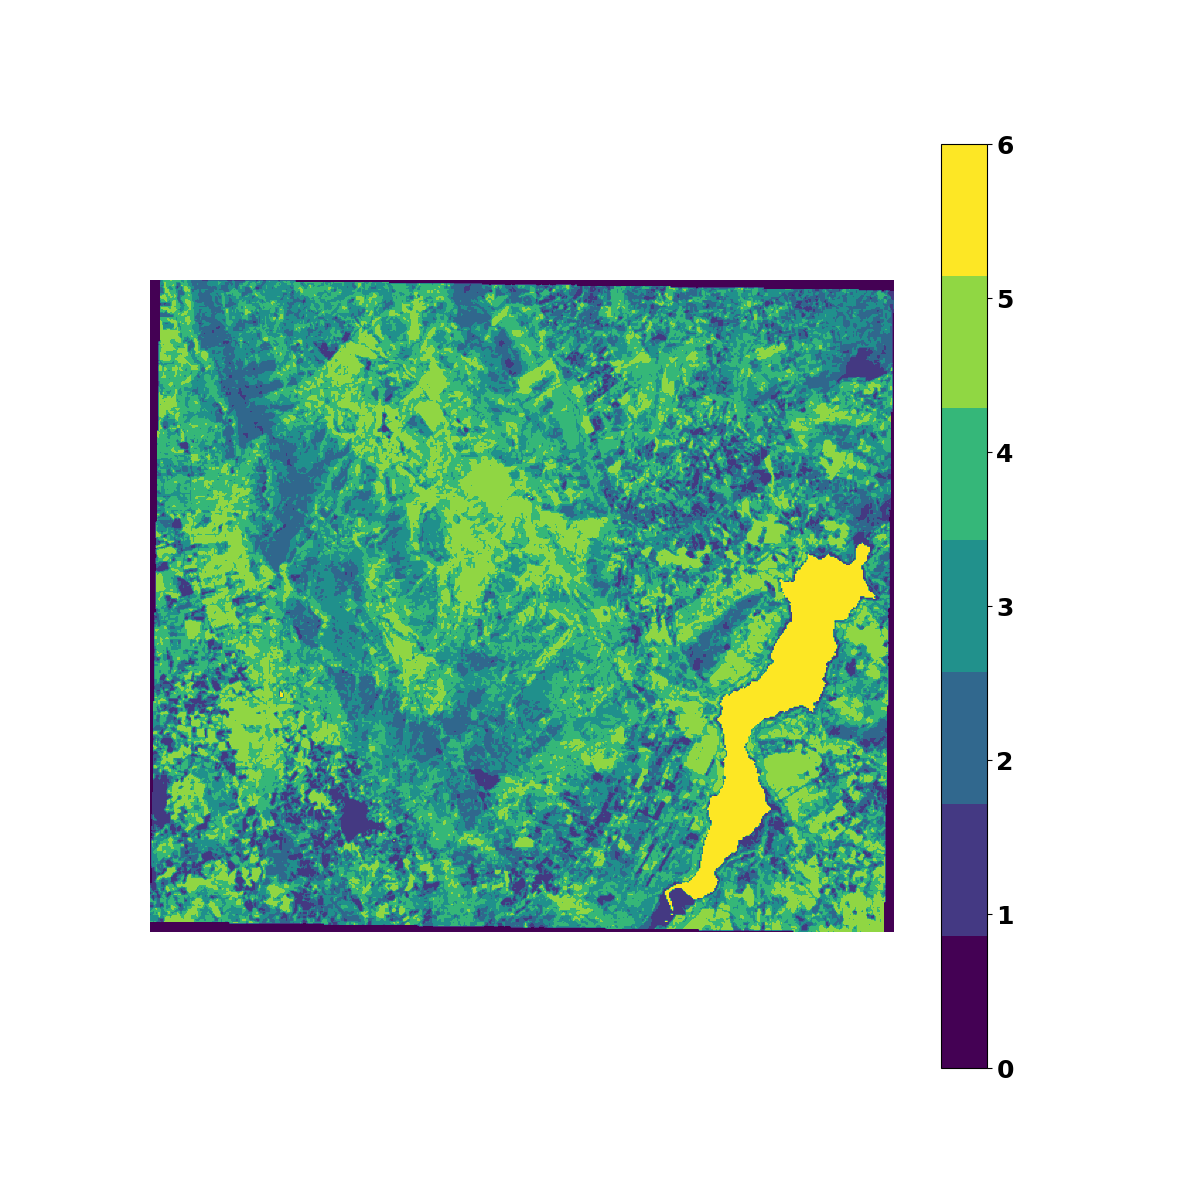
\includegraphics[width=\textwidth]{images/results/april/case/Riserva naturale Pizzo Cane, Pizzo Trigna, Grotta Mazzamuto_K=6+1_2017_april.png}
      \caption{Case study — Drought conditions in April 2017}
      \label{fig:case_april_lr_2017}
  \end{minipage}
  \hfill
  \begin{minipage}{1\columnwidth}
      \centering
      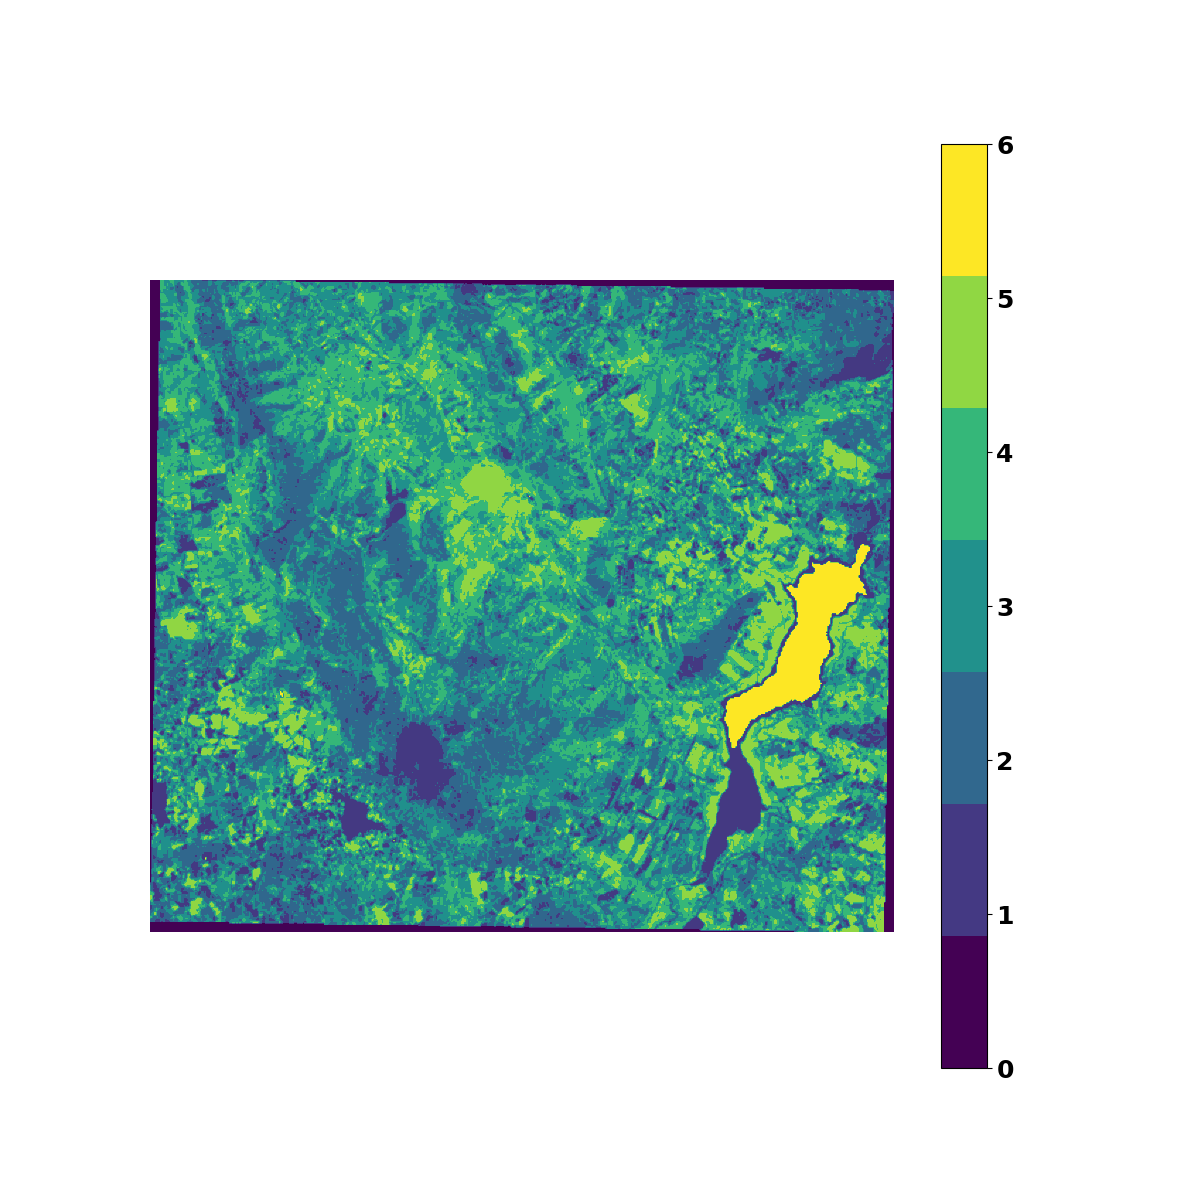
\includegraphics[width=\textwidth]{images/results/april/case/Riserva naturale Pizzo Cane, Pizzo Trigna, Grotta Mazzamuto_K=6+1_2024_april.png}
      \caption{Case study — Drought conditions in April 2024}
      \label{fig:case_april_lr_2024}
  \end{minipage}

\end{figure*}


\begin{figure*}[h]
  \centering

  \begin{minipage}{1\columnwidth}
      \centering
      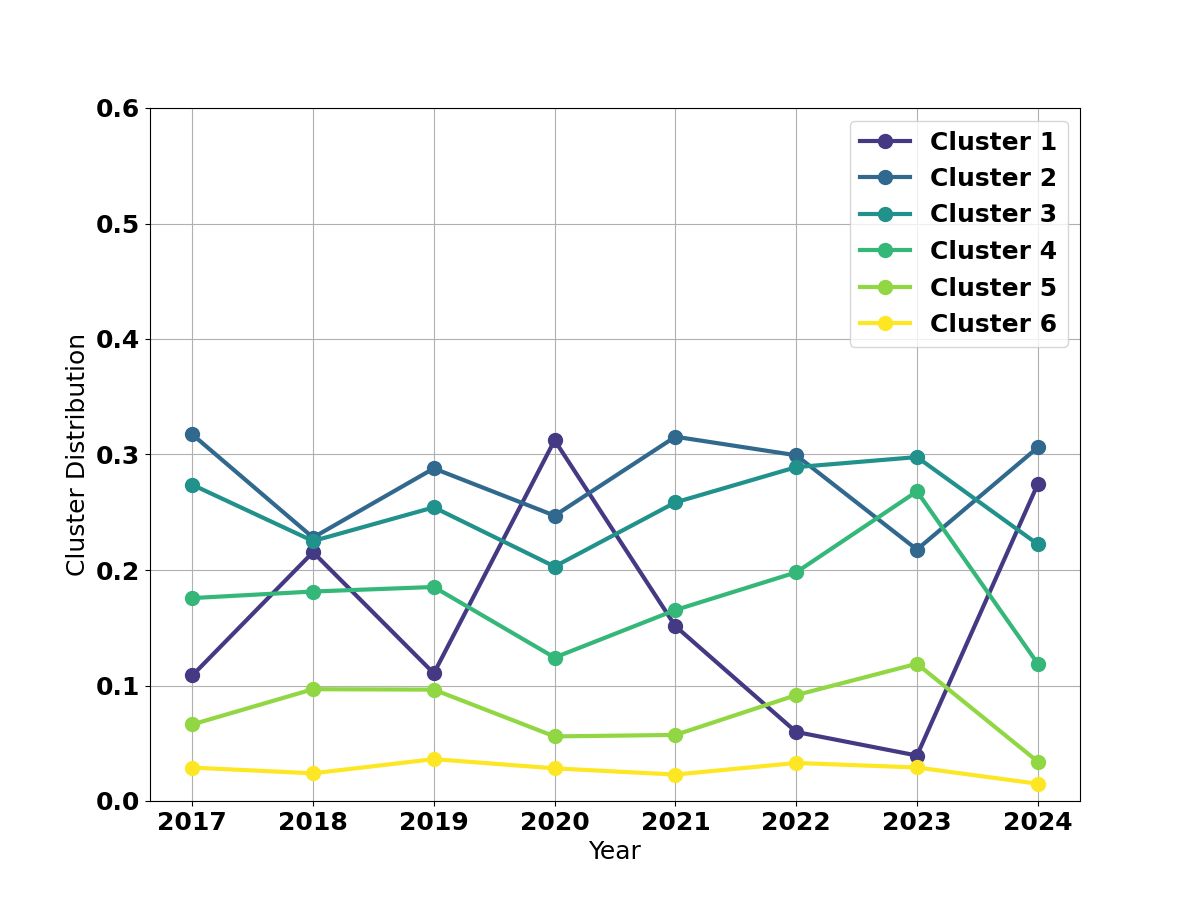
\includegraphics[width=\textwidth]{images/results/july/case/cluster_distribution_6_july.png}
      \caption{Case study - Cluster distribution in July 2017-2024}
      \label{fig:case_july_clust_dist}
  \end{minipage}
  \hfill
  \begin{minipage}{1\columnwidth}
      \centering
      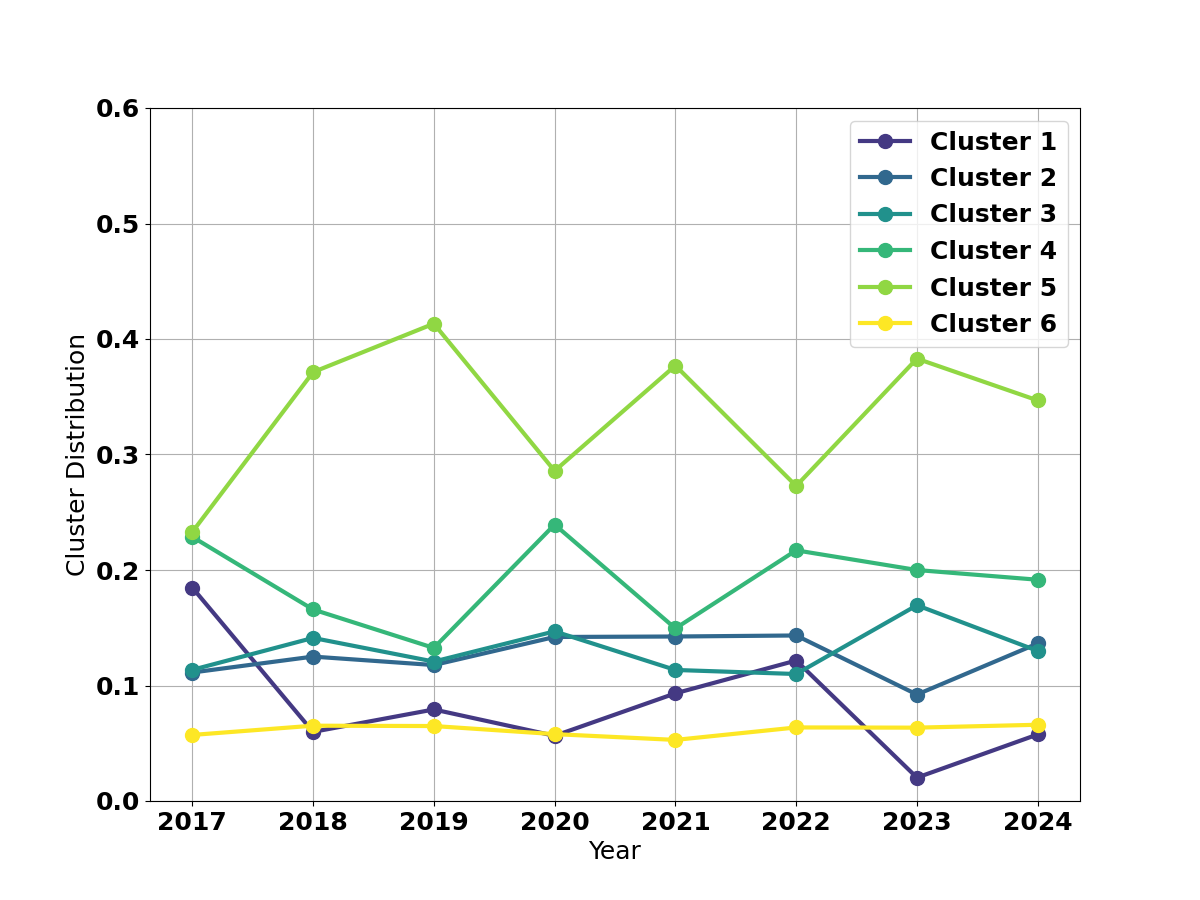
\includegraphics[width=\textwidth]{images/results/july/control/cluster_distribution_6_july.png}
      \caption{Control study - Cluster distribution in July 2017-2024}
      \label{fig:control_july_clust_dist}
  \end{minipage}

\end{figure*}


\begin{figure*}[h]
  \centering

  \begin{minipage}{1\columnwidth}
      \centering
      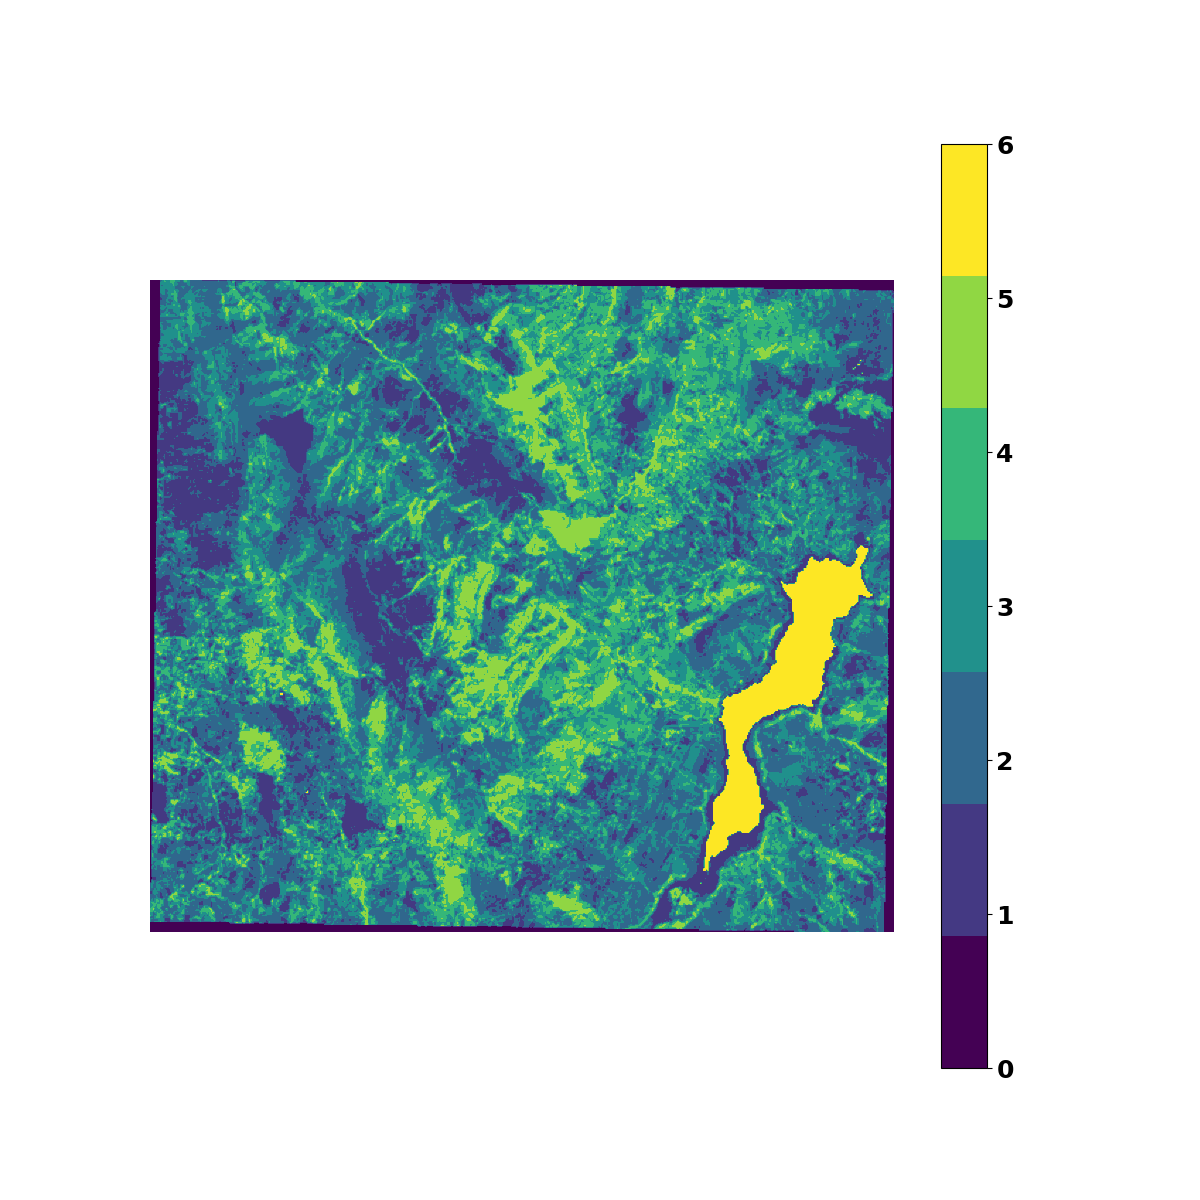
\includegraphics[width=\textwidth]{images/results/july/case/Riserva naturale Pizzo Cane, Pizzo Trigna, Grotta Mazzamuto_K=6+1_2017_july.png}
      \caption{Case study — Drought conditions in July 2017}
      \label{fig:case_july_lr_2017}
  \end{minipage}
  \hfill
  \begin{minipage}{1\columnwidth}
      \centering
      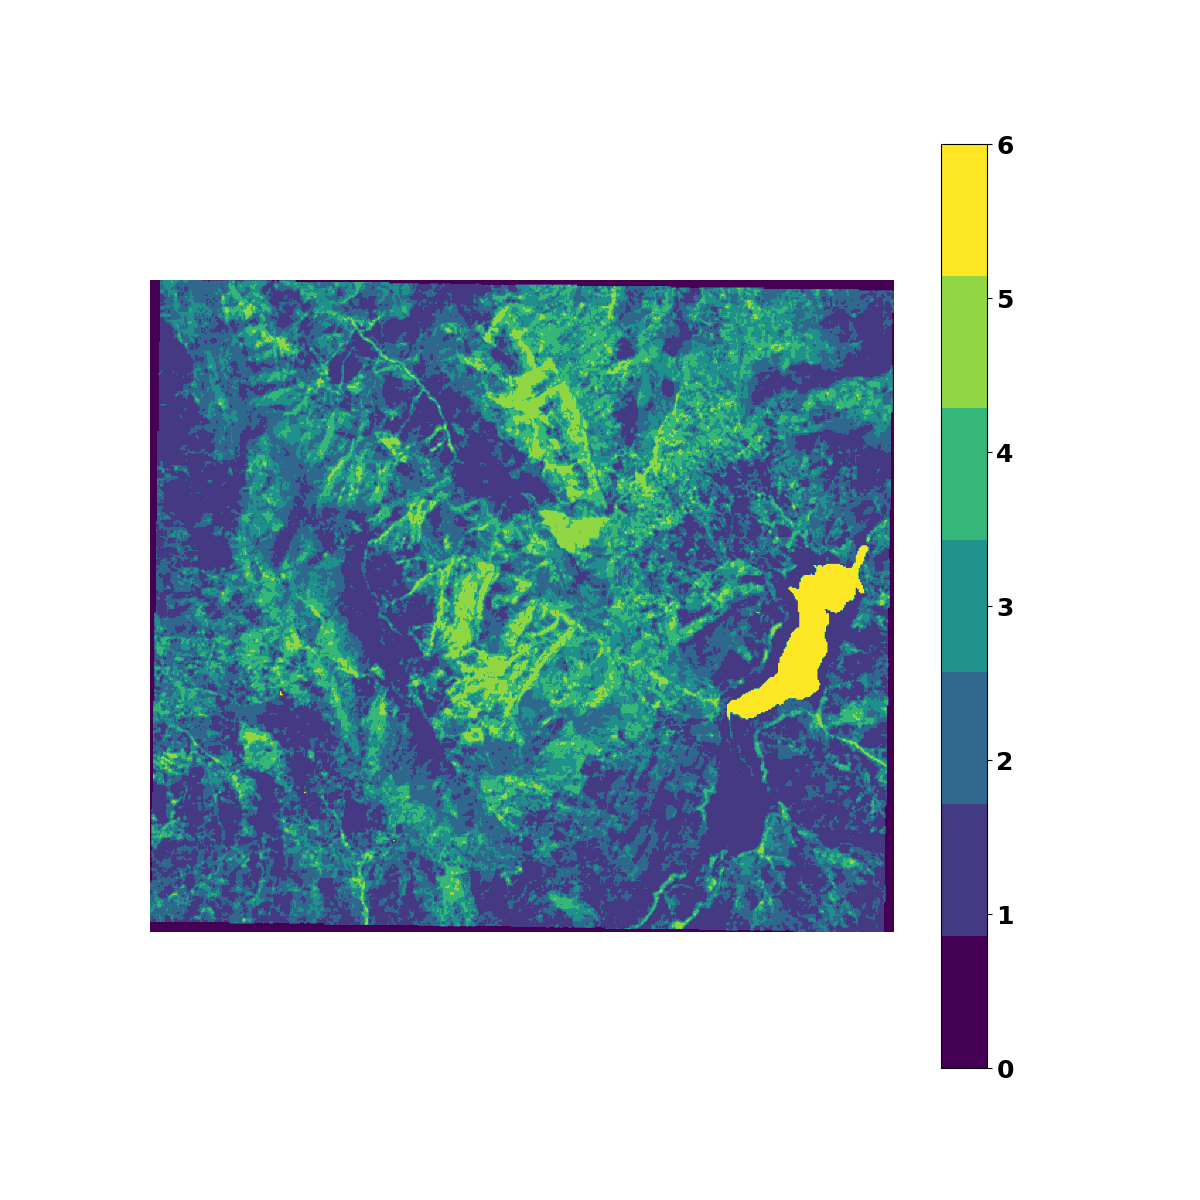
\includegraphics[width=\textwidth]{images/results/july/case/Riserva naturale Pizzo Cane, Pizzo Trigna, Grotta Mazzamuto_K=6+1_2024_july.png}
      \caption{Case study — Drought conditions in July 2024}
      \label{fig:case_july_lr_2024}
  \end{minipage}

\end{figure*}
\end{document}